\documentclass[11pt]{beamer}
\usetheme{Copenhagen}
\usepackage[utf8]{inputenc}
\usepackage{amsmath}
\usepackage{amsfonts}
\usepackage{amssymb}
\usepackage[font=small,labelfont=bf]{caption}
\usepackage{hyperref}
\usepackage{xcolor}

\newcommand{\blue}[1]{\textcolor{blue}{#1}}

\author{LAURENT Louis}
\title{Cours Container}
%\setbeamercovered{transparent} 
\setbeamertemplate{navigation symbols}{}
\date{2021-03-23}

\begin{document}

\begin{frame}
\titlepage
\end{frame}

\begin{frame}{Table des matières}
\tableofcontents
\end{frame}

\AtBeginSection[]
{
  \begin{frame}
    \frametitle{Table des matières}
    \tableofcontents[currentsection]
  \end{frame}
}

\section{Introduction}
\begin{frame}{Problématique}
Pourquoi les outils de virtualisation et conteneurisation existent ?
\end{frame}

\begin{frame}{Virtualisation}
\begin{block}{Définition}
La virtualisation a pour objectif la simulation de composant ou de service sur un matériel existant. Pour y parvenir il utilise un hyperviseur.
\end{block}
\end{frame}

\begin{frame}{Virtualisation}
\begin{columns}
    \begin{column}{0.48\textwidth}
        \begin{figure}
			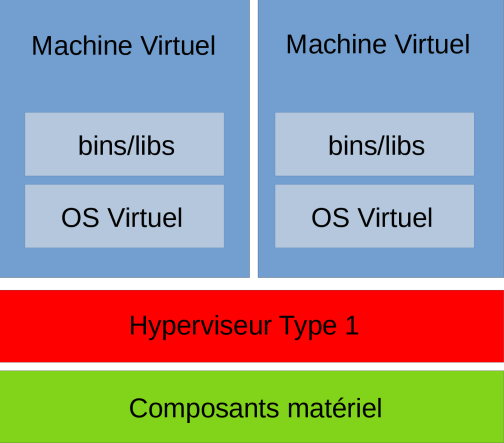
\includegraphics[scale=0.30]{images/type1.png}
			\caption{Hyperviseur de type 1}
		\end{figure}
    \end{column}
    \begin{column}{0.48\textwidth}
        \begin{figure}
			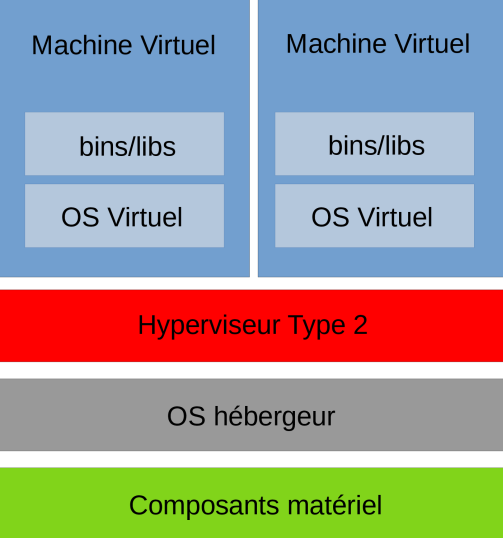
\includegraphics[scale=0.25]{images/type2.png}
			\caption{Hyperviseur de type 2}
		\end{figure}
    \end{column}
\end{columns}

\end{frame}

\begin{frame}{Conteneurisation}
\begin{block}{Définition}
La conteneurisation est une méthode de virtualisation qui utilise le système d'exploitation de l'hôte comme base pour ses containers. Il utilise un moteur de conteneurisation.
\end{block}

\end{frame}

\begin{frame}{Conteneurisation}
	\begin{figure}
		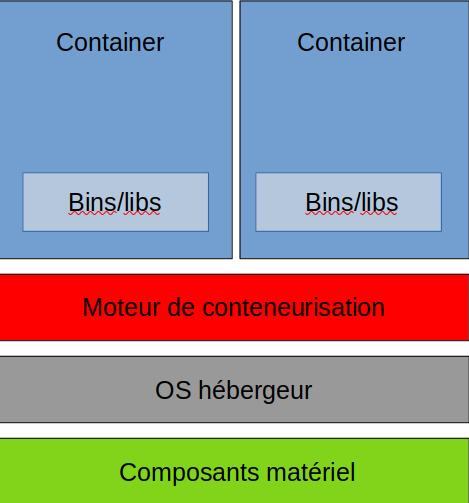
\includegraphics[scale=0.30]{images/container.png}
		\caption{Conteneurisation}
	\end{figure}
\end{frame}

\begin{frame}{Conteneurisation}
\begin{columns}
    \begin{column}{0.33\textwidth}
        \begin{figure}
			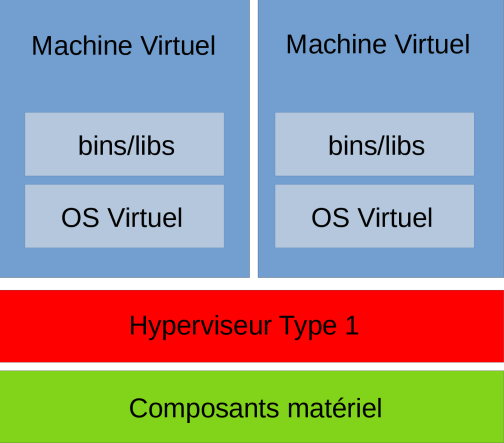
\includegraphics[scale=0.20]{images/type1.png}
			\caption{Hyperviseur de type 1}
		\end{figure}
    \end{column}
    \begin{column}{0.33\textwidth}
        \begin{figure}
			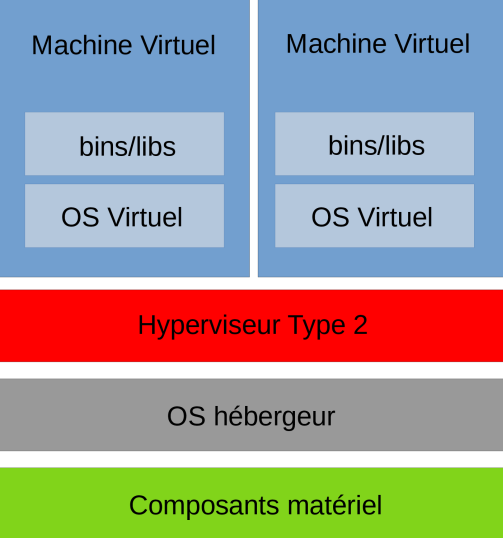
\includegraphics[scale=0.20]{images/type2.png}
			\caption{Hyperviseur de type 2}
		\end{figure}
    \end{column}
    \begin{column}{0.33\textwidth}
        \begin{figure}
			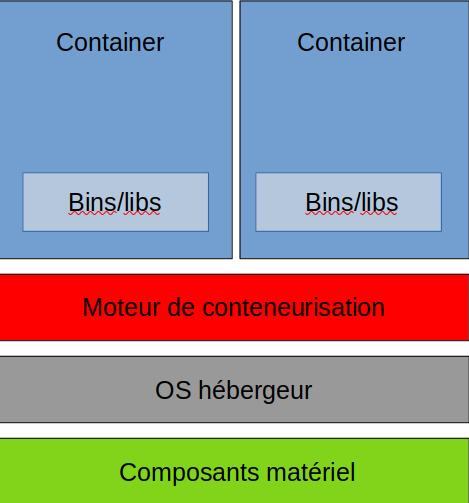
\includegraphics[scale=0.20]{images/container.png}
			\caption{Conteneurisation}
		\end{figure}
    \end{column}
\end{columns}

\end{frame}

\section{Écosystème}
\begin{frame}{Moteur de conteneurisation}
\begin{columns}
	\begin{column}{0.48\textwidth}
		\begin{figure}
			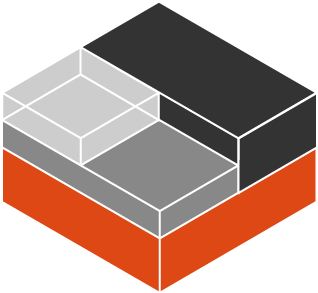
\includegraphics[scale=0.15]{images/lxd.png}
			\caption{LXC}
		\end{figure}
	\end{column}
	\begin{column}{0.48\textwidth}
		\begin{figure}
			
\includegraphics[scale=0.60]{images/containerd.png}
		\end{figure}
	\end{column}
\end{columns}

\end{frame}

\begin{frame}{Clients}
\begin{columns}
	\begin{column}{0.33\textwidth}
		\begin{figure}
			
\includegraphics[scale=0.10]{images/docker.png}
		\end{figure}
	\end{column}
	\begin{column}{0.33\textwidth}
		\begin{figure}
			
\includegraphics[scale=0.15]{images/podman.png}
		\end{figure}
	\end{column}
	\begin{column}{0.33\textwidth}
		\begin{figure}		
			
\includegraphics[scale=0.20]{images/portainer.png}
		\end{figure}	
	\end{column}
\end{columns}

\end{frame}

\begin{frame}{Écosystème}
\begin{columns}
	\begin{column}{0.33\textwidth}
		\begin{figure}
			
\includegraphics[scale=0.20]{images/docker_compose.png}
		\end{figure}	
	\end{column}
	\begin{column}{0.33\textwidth}
		\begin{figure}
			
\includegraphics[scale=0.25]{images/kubernetes.png}
		\end{figure}	
	\end{column}\
	\begin{column}{0.33\textwidth}
		\begin{figure}
			
\includegraphics[scale=0.04]{images/openshift.png}
		\end{figure}	
	\end{column}
\end{columns}

\end{frame}

\section{Docker}
\begin{frame}{Fonctionnement}
	\begin{figure}
		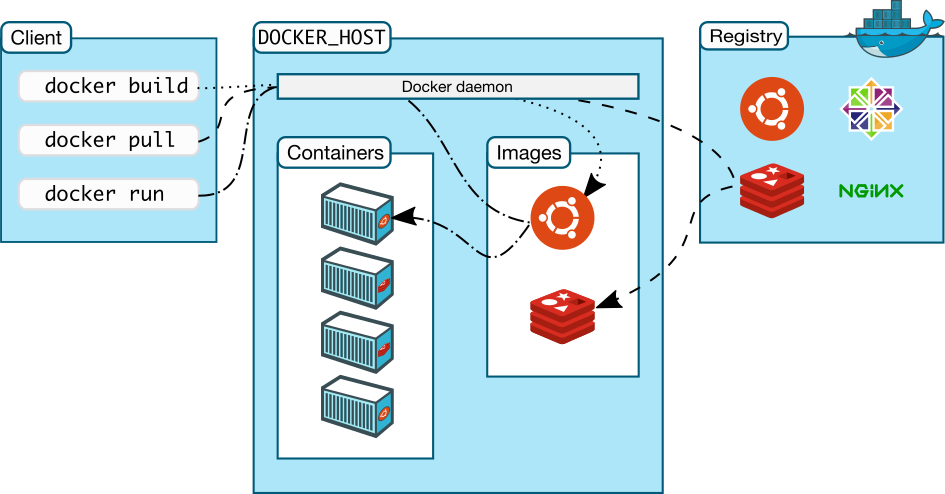
\includegraphics[scale=0.25]{images/docker_architecture.png}
	\end{figure}
\end{frame}

\begin{frame}{Installation}
	\begin{itemize}
		\item \href{https://docs.docker.com/docker-for-windows/install/}{\blue{\underline{Windows}}}
		\item \href{https://docs.docker.com/engine/install/debian/}{\blue{\underline{Linux}}}
	\end{itemize}
\end{frame}

\begin{frame}{Comment docker fonctionne en pratique ?}
	\begin{itemize}
		\item Dockerfile
		\item Container
		\item Network
		\item Volume
	\end{itemize}
\end{frame}

\begin{frame}{Dockerfile}
	\begin{figure}
		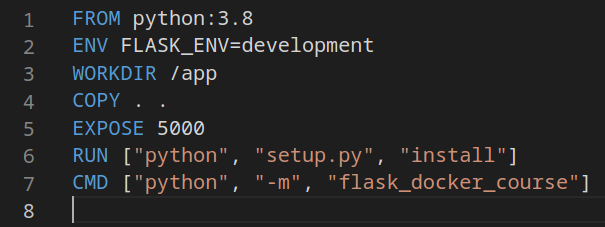
\includegraphics[scale=0.5]{images/dockerfile.png}
	\end{figure}

\end{frame}

\begin{frame}{Dockerfile Multi-Stages Build}
	\begin{figure}
		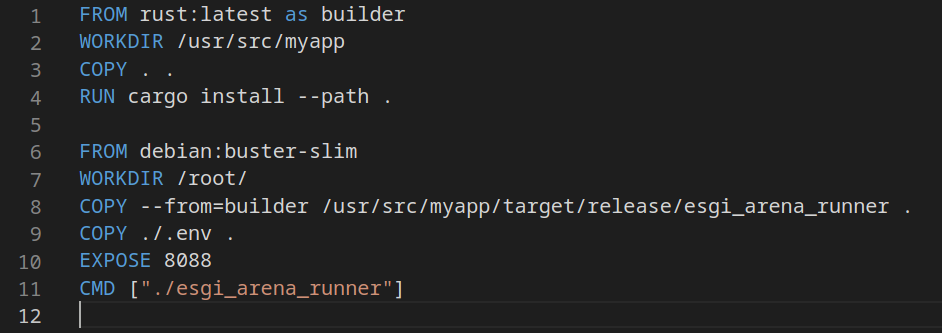
\includegraphics[scale=0.4]{images/dockerfile_multi.png}
	\end{figure}

\end{frame}

\begin{frame}{Utilisation}
	\centering
	\frame{\href{https://youtu.be/RP40sWR-4Rc}{
		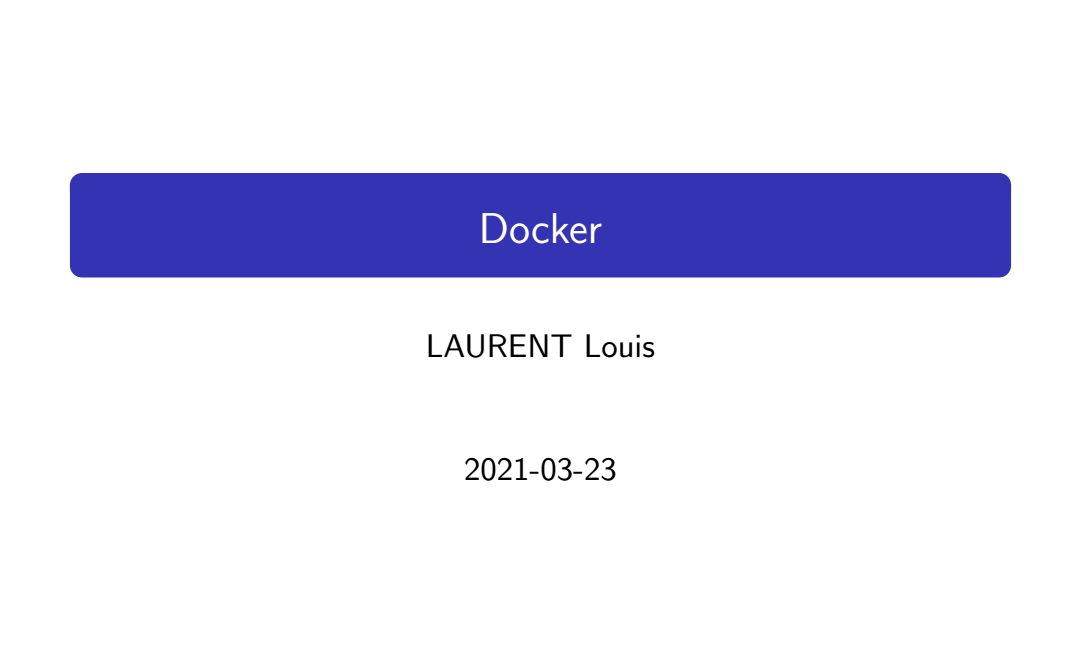
\includegraphics[width=\textheight, keepaspectratio]{images/video_docker.png}
	}}
	
\end{frame}

\begin{frame}{Commandes utiles}
	\begin{figure}
		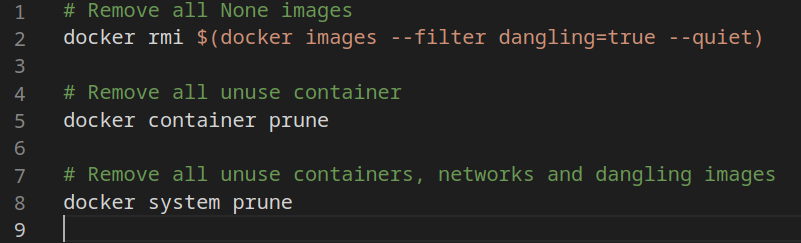
\includegraphics[scale=0.45]{images/commandes_pratiques.png}
	\end{figure}

\end{frame}

\section{Docker Compose}
\begin{frame}{Installation}
	\begin{itemize}
		\item \href{https://docs.docker.com/compose/install/}{\blue{\underline{Windows/Linux}}}
	\end{itemize}

\end{frame}

\begin{frame}{Utilisation}
	\centering
	\frame{\href{https://youtu.be/9GLExiJu9jY}{
		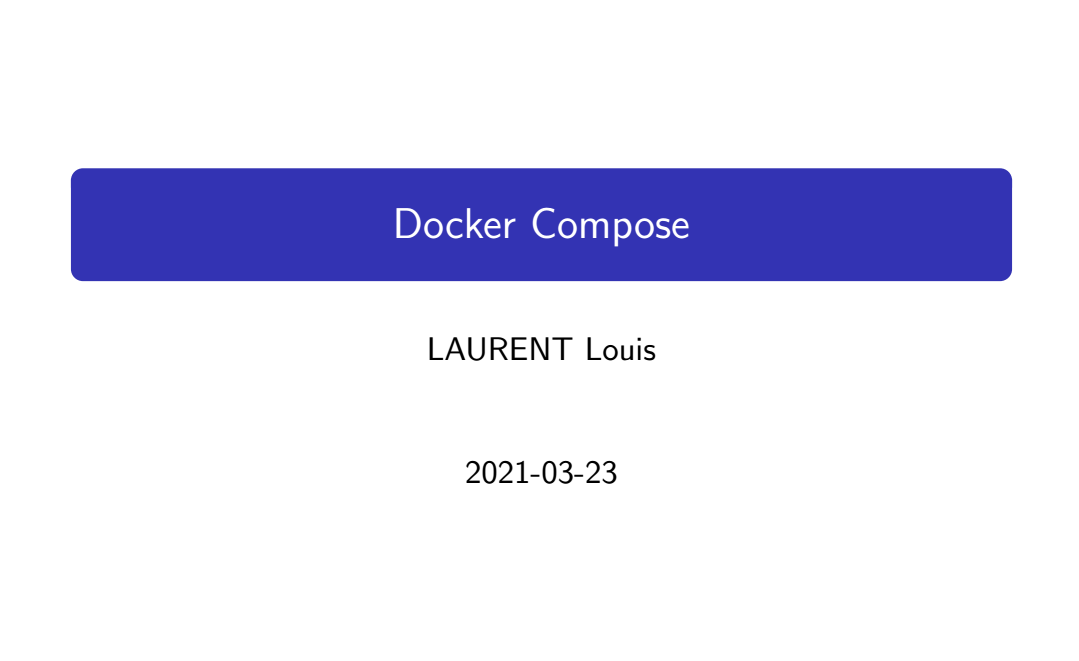
\includegraphics[width=\textheight, keepaspectratio]{images/video_docker_compose.png}
	}}
	
\end{frame}

\section{Resources}
\begin{frame}
	\begin{itemize}
		\item \href{https://docs.docker.com/get-started/overview/}{\blue{\underline{Docker}}}
		\item \href{https://podman.io/}{\blue{\underline{Podman}}}
		\item \href{https://www.portainer.io/}{\blue{\underline{Portainer.io}}}
		\item \href{https://containerd.io}{\blue{\underline{Containerd}}}
		\item \href{https://opencontainers.org/}{\blue{\underline{Open Container Initiative}}}
		\item \href{https://linuxcontainers.org/fr/}{\blue{\underline{LXC}}}
		\item \href{https://kubernetes.io/fr/}{\blue{\underline{Kubernetes}}}
		\item \href{https://www.openshift.com/}{\blue{\underline{OpenShift}}}
		\item \href{https://github.com/ulphidius/flask_docker_course}{\blue{\underline{Code Source}}}
	\end{itemize}

\end{frame}

\end{document}